%%%%%%%%%%%%%%%%%%%%%%%%%
%%  Capítulo 3: Modelado y simulacion de metamateriales  %%
%%%%%%%%%%%%%%%%%%%%%%%%%

%%%%
\section{Análisis de estructuras periódicas}
\label{sec_estructuras_periodicas}
%%%%
\lipsum
% Libro de rahmat. Pagina 59.
%%%%
\section{Análisis de estructuras planares propuestas}
\label{sec_estructuras_propuestas}
%%%%
\lipsum
\lipsum
% Comentar cómo se logró periodicidad, vinculando las fases.
%%%%
\section{Estudio de estructuras mediante TLM}
\label{sec_estudio_tlm}
%%%%
\lipsum
%Pasos: Barchloui: Simulation of FSS surfaces using 3d TLM, 2003. Primer paper de un librito. Buena explciaci{on.}
% Paper importante: Hoefer 1985. Johns, 1971.
% Leer Janyani, Paul, TLM modelling of nonlinear optical effects in fibre bragg gratings, 2004.
% Kim Kim Kang, Yook: Modeling and analysis of ebg in power distribution networks.
% sadiku
		
%%%%
\subsection{Algoritmo utilizando programación orientada a objetos}
\label{subsec_estudio_tlm}
%%%%
La simulación se corre a través de un \textit{script} editable de Python, donde se establecen las condiciones de la simulación en forma manual, y se determina si se leerán resultados calculados previamente o se calcularán nuevos. En el mismo, además, se permite elegir si se considerarán  las capacidades de acople entre elementos, la cantidad de tiempos a simular y las frecuencias superior e inferior de análisis. Se debe tener en cuenta, además, que se especifica la discretización espacial (cantidad de milímetros de cada estructura simulada, denominada \textit{Pixel}). La discretización espacial se relaciona con la temporal, dado que en TLM están vinculadas por la velocidad de propagación de una onda electromagnética en el medio. Así, la primera deberá asegurar que la segunda permita cumplir con las condiciones del teorema de Nyquist para la caracterización de las señales calculadas (esto significa que, dado que la velocidad de propagación, $v_p=\frac{\Delta l}{\Delta t}$ relaciona las discretizaciones espacial y temporal, la discretización espacial debe ser tal que $\Delta l = v_p \frac{\Delta t}{2}$ para cumplir las condiciones del teorema de Nyquist, lo que deriva en que $\Delta l = \frac{v_p}{2f}$, con $f$ la frecuencia de interés, que en nuestro caso es $2.4\;GHz$).

\begin{figure}[h]
	\centering
	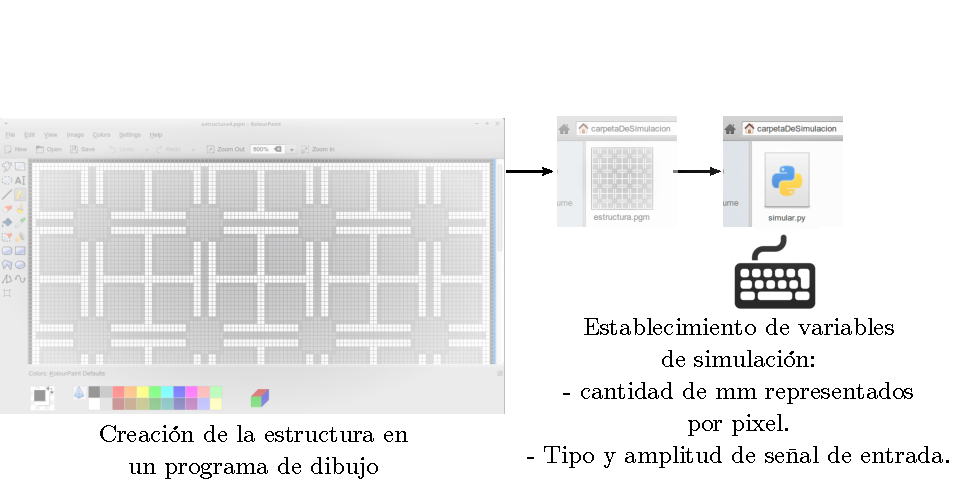
\includegraphics[width=\textwidth]{Modelado/ProcedimientoUsuario.pdf}
	\caption{Esquema de ingreso de datos al simulador.}
	\label{fig:esquema-ingreso-datos}
\end{figure}

Como se esquematiza en la figura \ref{fig:esquema-ingreso-datos}, la entrada de datos se realiza a través de un archivo con formato \textsc{.PGM}, que establece una matriz de \textit{pixeles}, cada uno con un valor, entre 1 y 255, donde 1 representa el negro, 255 el blanco, y los valores intermedios corresponden a una escala de grises. El archivo se puede generar a partir de un programa de edición de imágenes, lo que facilita la creación de estructuras a simular, ya que la misma sólo debe ser dibujada con la resolución requerida. Si la imagen creada ocupa una mayor cantidad de \textit{pixeles} (tiene una mayor resolución), la granularidad espacial utilizada en la simulación será mayor, dado que existe una relación 1 a 1 entre los \textit{pixeles} gráficos y la discretización utilizada.

La lectura de la imagen del disco genera un objeto \textit{Superficie}, que almacena, en forma ordenada, los \textit{Pixeles} dibujados, que son objetos con características eléctricas variables, en función de su color en la imagen, como se muestra en la figura \ref{fig:tiposdepixeles}. En la misma se pueden observar 4 tipos de \textit{pixeles}:

\begin{figure}[h]
	\centering
	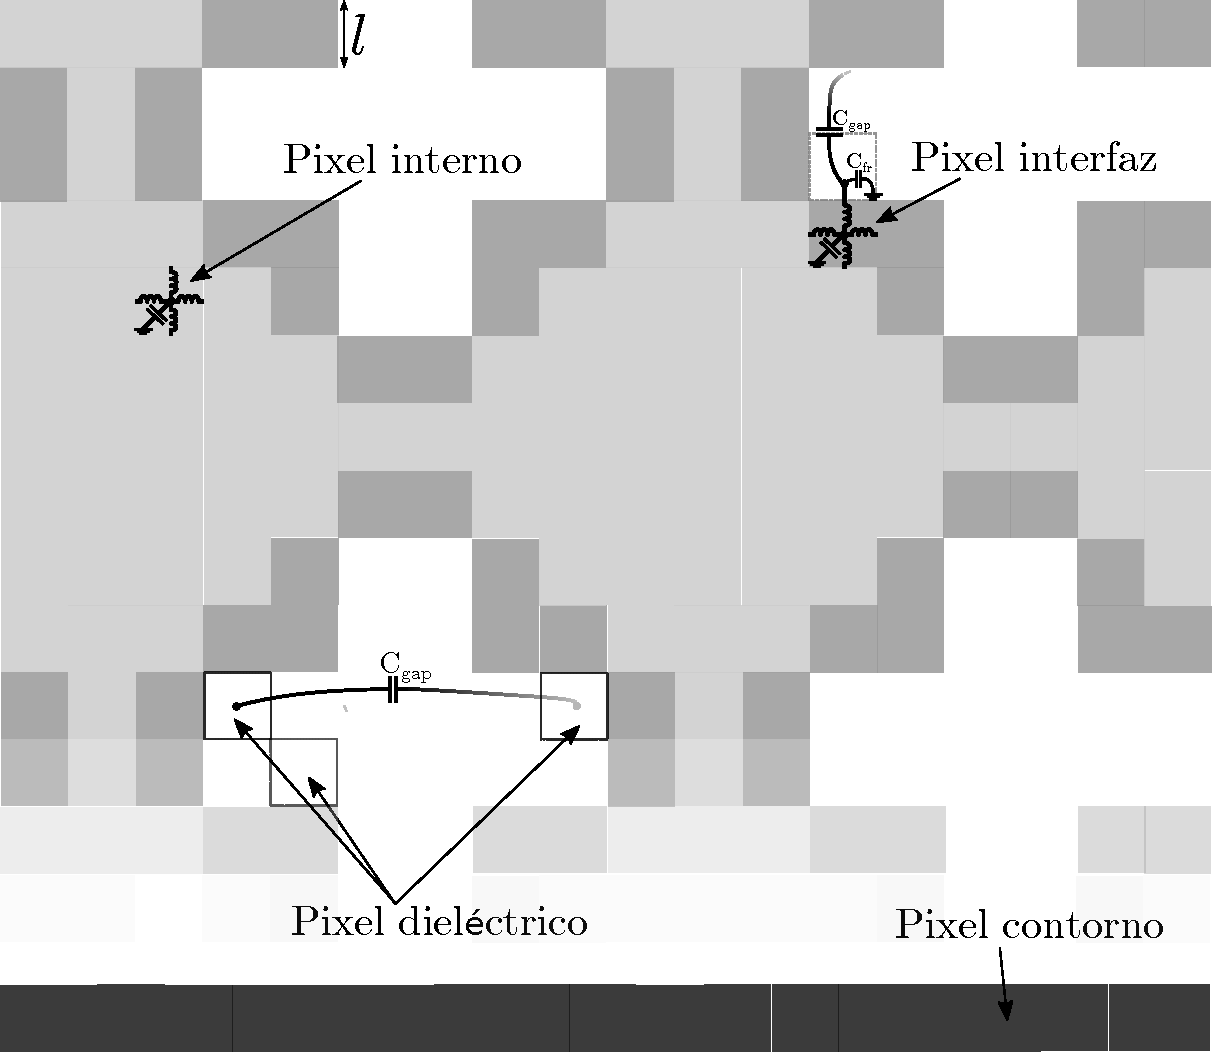
\includegraphics[width=\textwidth]{Modelado/TiposDePixel.pdf}
	\caption{Circuitos equivalentes propuestos para cada tipo de pixel.}
	\label{fig:tiposdepixeles}
\end{figure}

\begin{enumerate}
	\item \textbf{Interno}.Representan superficies metálicas que se encuentran en el interior de un plano conductor.
	\item \textbf{Interfaz}. Representan superficies metálicas que se encuentran en los bordes de una estructura metálica, lo que significa que tienen vecinos que son otros \textit{pixeles} de tipo metálico (de interfaz o internos) y vecinos dieléctricos. Son los \textit{pixeles} que poseen la propiedad de capacidad de \textit{fringe}.
	\item \textbf{Dieléctricos}. Representan las zonas donde no hay cobre, sino simplemente dieléctrico desnudo (en particular, FR4). Estos \textit{pixeles} no participan del intercambio de energía en el modelo.
	\item \textbf{Contorno}. Pueden intentar simular una superficie perfectamente adaptada, o una superficie metálica, en función de las necesidades de la simulación. Se ubican en el borde de la imagen \textsc{.pgm} creada, para que actúen como el borde del espacio de simulación.
\end{enumerate}


Una vez cargada la imagen en memoria, creado el objeto \textit{Superficie} y los objetos \textit{Pixeles}, se los vincula.

Como se observa en la figura \ref{fig:tiposdepixeles}, los pixeles metálicos (internos y de interfaz) tienen una capacidad y varias inductancias asociadas (una para cada dirección). Las mismas quedan descriptas en base a las ecuaciones \ref{eq:Cp_Lp}, y a partir de ellas es posible obtener una impedancia característica, como se muestra en la figura \ref{fig:modelo-con-lineas-de-transmision}, en base a las ecuaciones \ref{eq:capacidad-inductancia-impedancia-modelado}:

\begin{subequations}
	\label{eq:capacidad-inductancia-impedancia-modelado}
	\begin{align}
		L_{inn} &= \mu_0 h /2 \\
		C_{inn} &= \frac{\epsilon_r \epsilon_0 l^2}{h} \\
		Z_{inn} &= \sqrt{L_{inn} / C_{inn}}
	\end{align}
\end{subequations}

\begin{figure}[h]
	\centering
	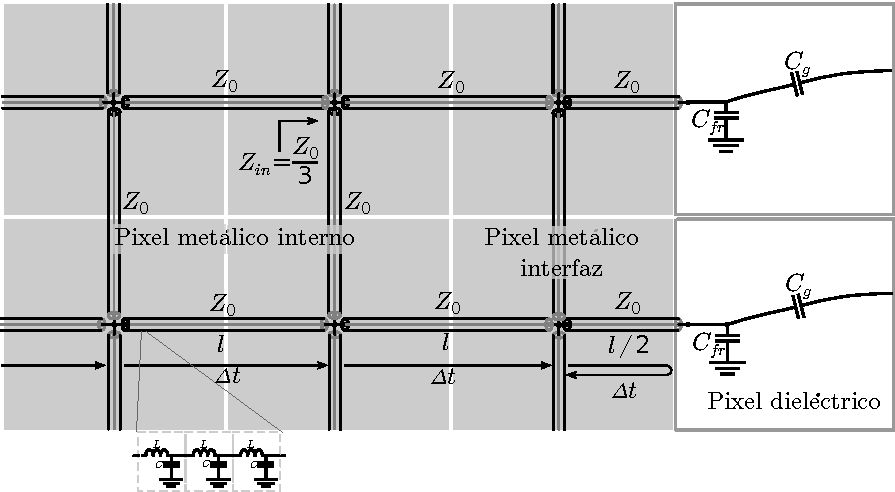
\includegraphics[width=0.8\textwidth]{Modelado/Modelo-Pixeles.pdf}
	\caption{Circuito equivalente de líneas de transmisión, donde se observa la relación con la capacidad e inductancia de cada \textit{Pixel}.}
	\label{fig:modelo-con-lineas-de-transmision}
\end{figure}

Los pixeles interfaz poseen, además, una capacidad de \textit{fringe}, que se relaciona al comportamiento no-TEM de las líneas de campo cerca de los bordes de las estructuras \textit{microstrip}, mostrado en la figura \ref{fig:microstrip-campos}. La expresión de la capacidad de \textit{fringe} para cada borde es la siguiente \cite{ThummWiesbeck:CharacteristicImpedance}, donde $u$ es la profundidad de metal para ese borde en cuestión, como se muestra en la figura \ref{fig:profundidad-para-cfringe}:

\begin{equation}
	C_{fr} = \frac{\epsilon_0 \epsilon_r} {\pi} \ln (2 \pi e^{\frac{u}{2 h} + 0.92})
\end{equation}

\begin{figure}[h]
	\centering
	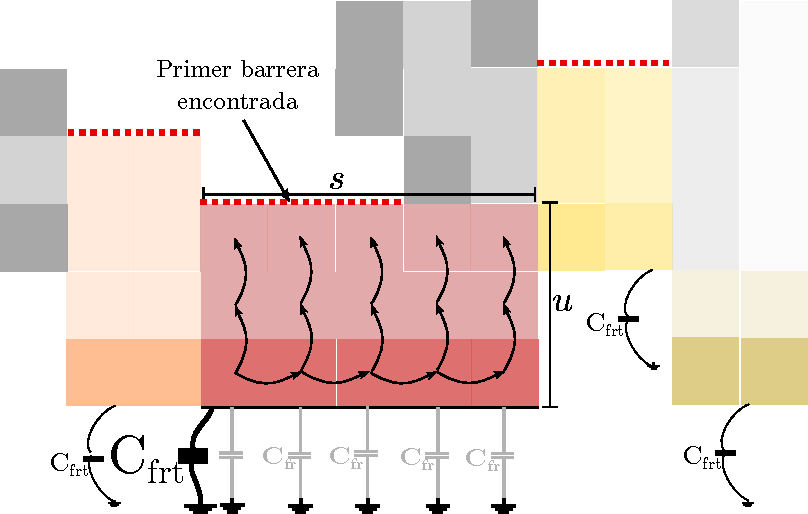
\includegraphics[width=0.8\textwidth]{Modelado/ProcesoCfringe.pdf}
	\caption{Cálculo de la capacidad de \textit{fringe} de una pared horizontal.}
	\label{fig:profundidad-para-cfringe}
\end{figure}

Al momento de crear la superficie, además, se realizan dos acciones previas a la simulación:

\begin{enumerate}
	\item \textbf{Vincular capacitivamente los bordes de las estructuras metálicas}, como se indica en la figura \ref{fig:calculoCapacidadTLM}. Para esto se toman todos los bordes de las estructuras metálicas (los pixeles de tipo \textit{Interfaz}), y se recorre horizontal y verticalmente la matriz, una vez por dirección, vinculando los bordes interfaz de a pares, teniendo en cuenta que aquellos \textit{pixeles} de interfaz que corresponden a la misma estructura (a la misma isla metálica) no deben ser vinculados.
	
	\begin{figure}[h]
		\centering
		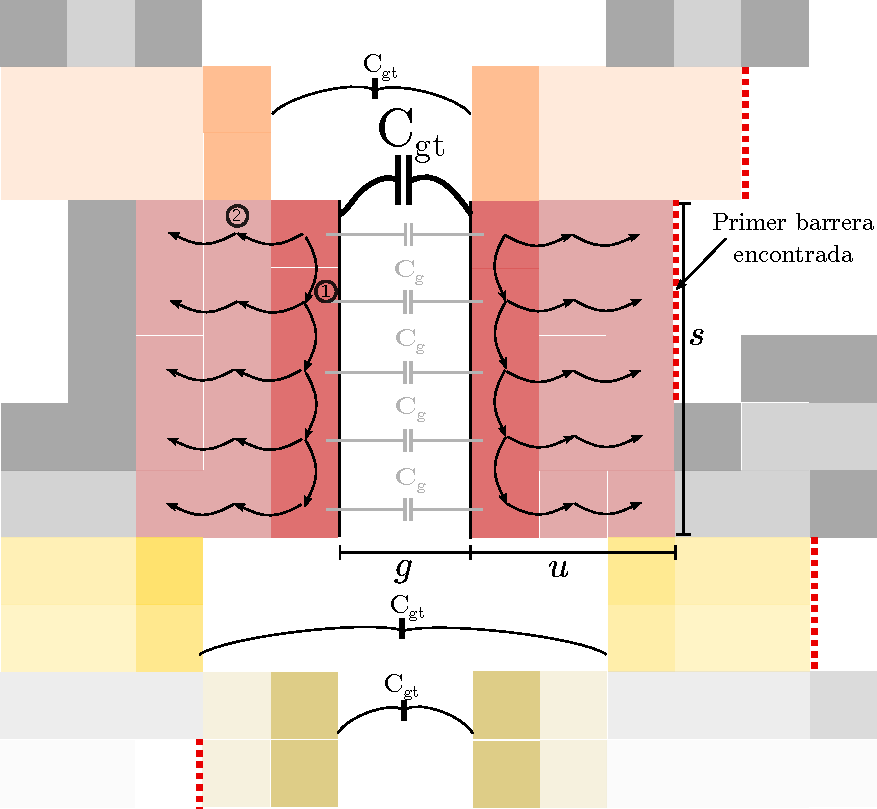
\includegraphics[width=0.9\textwidth]{Modelado/ProcesoProfundidad.pdf}
		\caption{Cálculo de las distintas capacidades de acople horizontales para los pixeles que participan del cálculo numérico. Para un caso particular se muestran las capacidades de acople asociadas a los pixeles enfrentados por un \textit{gap}.}
		\label{fig:calculoCapacidadTLM}
	\end{figure}
	
	Por cada par encontrado, se obtiene la capacidad de acople, $C_{gt}$, utilizando la expresión \ref{eq:cgap-y-lgap}, reescrita aquí para simplificar la lectura:
	
	\begin{align*}
		C_{gap} = \frac{b \epsilon_0 (1+\epsilon_r)}{\pi} \cosh^{-1} (a / g) \\
	\end{align*}
	
	En esta expresión, $a$ es el tamaño de las islas metálicas y $g$ representa la distancia entre las islas conductoras. El valor de $s$, en tanto, representa la longitud del $gap$, que se obtiene calculando la cantidad de \textit{pixeles} enfrentado a distancia constante que existen (paso 1 en la figura). Hecho esto, considerando todos los pixeles a uno y otro lado del \textit{gap}, se busca la "profundidad" de la celda, $u$, que no es más que la cantidad de pixeles metálicos detrás de los pixeles frontera que pueden hallarse simultáneamente a ambos lados del \textit{gap}, manteniendo al cantidad longitudinal de pixeles metálicos del borde (paso 2 en la figura). Así, el valor de $a$ queda representado por, aproximadamente, $2*u+g$, con $u$ en unidades de metro.
	
	El valor de la capacidad total de acople se divide entre la cantidad de pares de pixeles que participan del cálculo, de manera que a cada par se le asigna una capacidad $C_g$, como se indica en la figura para los pixeles de color rojo.
	
	\item \textbf{Calcular las matrices S asociadas a cada pixel metálico.} Las matrices S son las matrices que, multiplicadas por un vector de tensiones incidentes, $V_i$ a cada pixel, devuelven un vector de igual dimensión de tensiones reflejadas, $V_r$ en los mismos, como se muestra en la ecuación \ref{eq:multiplicacion-matriz-s}. Cada uno de los elementos de estos vectores representan una dirección (izquierda, derecha, arriba y abajo) de la celda unitaria. Las expresiones de la matriz S son las mostradas en la ecuación \ref{eq:matriz-s-expresiones}:
	
	\begin{align}
		\label{eq:multiplicacion-matriz-s}
		\begin{bmatrix}
			V_r^{izq} \\
			V_r^{der} \\
			V_r^{arr} \\
			V_r^{aba} \\
		\end{bmatrix}
			=
		\begin{bmatrix}
			s_{izq-izq} & s_{der-izq} & \dots & \dots \\
			s_{izq-der} & s_{der-der} & \ddots & \vdots \\
			\vdots & \ddots & \ddots     & \vdots \\
			s_{izq-izq-aba} & \dots & \dots & s_{aba-aba}
		\end{bmatrix}
		\begin{bmatrix}
			V_i^{izq} \\
			V_i^{der} \\
			V_i^{arr} \\
			V_i^{aba} \\
		\end{bmatrix}
	\end{align}
	
	\begin{subequations}
		\label{eq:matriz-s-expresiones}
		\begin{align}
			S_{i,i} = \frac{Z_{j}||Z_{k}||Z_{l} -Z_{i}}{Z_{j}||Z_{k}||Z_{l} +Z_{i}} \\
			S_{j,i} = \frac{2 Z_{j}||Z_{k}||Z_{l}}{Z_{j}||Z_{k}||Z_{l} +Z_{i}}
		\end{align}
	\end{subequations}
	
	Se debe tener en cuenta que, para el caso de las líneas de transmisión que unen \textit{pixeles} metálicos (\textit{internos} y de \textit{interfaz}), como se muestra en la figura \ref{modelo-con-lineas-de-transmision}, cada una de las 4 líneas de transmisión que confluyen en un nodo representante de un pixel son iguales, por lo que el valor de los elementos de la diagonal de la matriz S será $-0.5$, mientras que los elementos no diagonales valdrán $0.5$.
	
	Además, se pueden establecer pérdidas para el transporte de tensión de un \textit{pixel} a otro, de manera que se puedan simular, de forma simplificada, las pérdidas por conductividad.
	
	Los \textit{pixeles} de tipo \textit{dieléctrico} no poseen matriz S, debido a que en su mayoría no tendrán información de tensión incidente.
\end{enumerate}

% explicar cómo se calcula cuando hay fringe
% explicar el acoplamiento

Para el análisis de transferencia entre un punto y otro de la estructura, se debe fijar una posición de entrada y una posición de salida, cuya tensión, para cada tiempo, deberá ser almacenada.

Una vez creada la matriz a partir de la información obtenida de la imagen, se debe establecer una tensión inicial en el nodo de entrada. Se puede establecer un $\delta(t)$ de tensión, de manera que se fija el valor de tensión inicial y luego se lo deja libre para todos los tiempos posteriores. También puede establecerse un seno y un pulso Gaussiano, que permite una excitación limitada en frecuencia \cite{Barthia:Handbook}.

La simulación es de tipo TLM, donde existe una tensión inicial impuesta para $t=0$, y elegida previamente al cálculo. A partir de la tensión ubicada en uno de los nodos, se calcula, en cada tiempo discreto, el valor de las tensiones incidentes a cada nodo, y a partir de las mismas, se calculan las tensiones reflejadas en todas las direcciones (\textit{scattering}), sumándose los efectos en todas ellas.

Así, como se muestra en la figura \ref{fig:procedimiento-tlm}, si se inicia el cálculo en el nodo denominado $a$, se impondrá una tensión inicial en el mismo, que será la que se transmita a los nodos adyecentes ($t_{1_b}$), denominados $b_i$. Esta tensión será recibida por los nodos $b_i$, quienes multiplicarán las tensiones incidentes en todas las direcciones (en el tiempo $t_{2_a}$, los nodos $b$ sólo tienen una dirección de incidencia) por su matríz $S$ asociada, para obtener las tensiones reflejadas y transmitidas. Estas tensiones, en el tiempo siguiente ($t_{2_b}$) son las que se transmiten a los respectivos nodos adyacentes, $c_j$, quienes repetirán la operación. El cálculo proseguirá hasta que se interrumpa la simulación.

\begin{figure}[h]
	\centering
	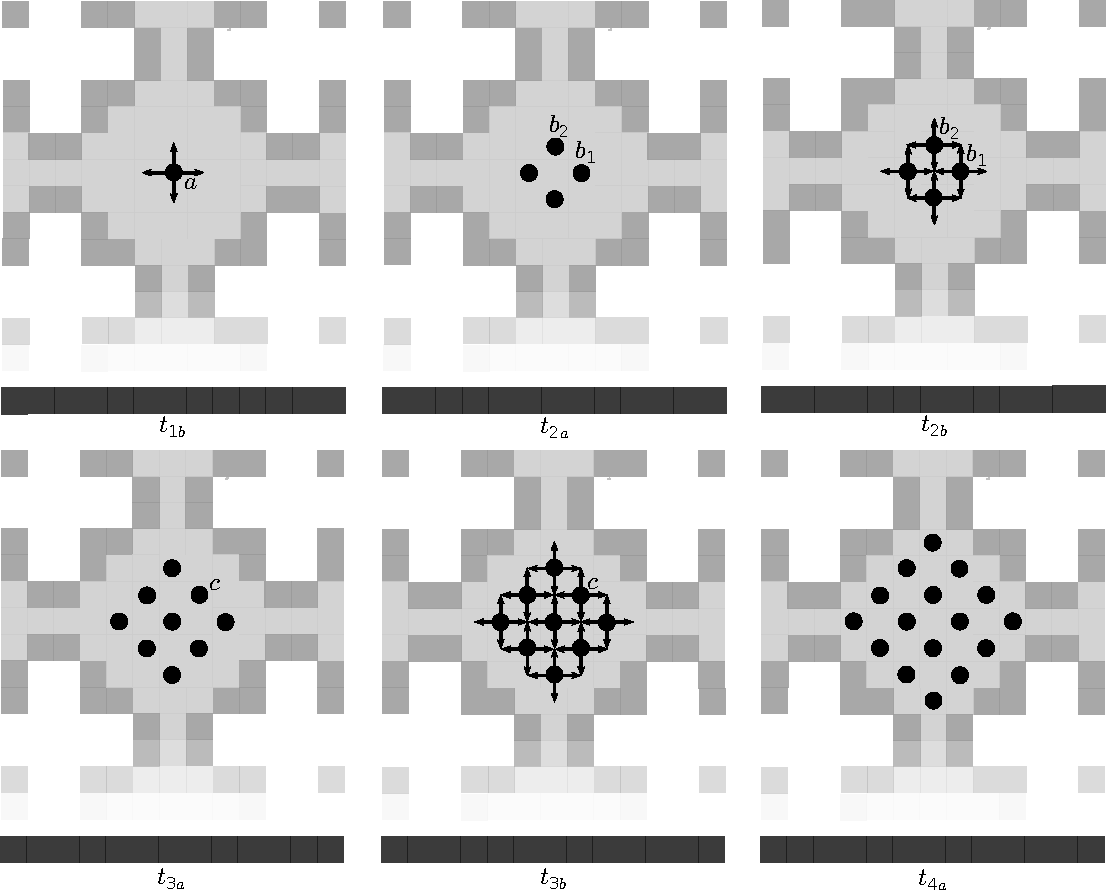
\includegraphics[width=0.9\textwidth]{Modelado/TLM-progresion.pdf}
	\caption{Proceso de cálculo en el dominio del tiempo.}
	\label{fig:procedimiento-tlm}
\end{figure}

Para el caso particular de los \textit{pixeles} de tipo \textit{interfaz}, existen dos situaciones especiales: La correspondiente al efecto de la capacidad de \textit{fringe} y el truncamiento de la línea de transmisión, y el correspondiente al acoplamiento con otras estructuras de la \textit{Superficie}.

Dado que el análisis es cuasiestático, debido a las dimensiones pequeñas de los \textit{gaps} y los Pixeles en comparación con la longitud de onda, se puede utilizar un modelo de bajas frecuencias de acoplamiento mutuo para describir el fenómeno de acoplamiento entre islas metálicas distintas. Este acoplamiento, en términos generales, se da por fenómenos inductivos y capacitivos al mismo tiempo. Si se considera que existe un elemento fuente y un elemento víctima del acoplamiento, se puede afirmar que cada uno de ellos expone una capacidad y una inductancia al ambiente, que son excitadas por los circuitos cercanos. El acoplamiento inductivo se debe a la inductancia mutua $M$ entre las inductancias expuestas de ambos, relacionada al campo magnético presente, mientras que el acoplamiento inductivo se debe a la capacidad de acople entre los circuitos ($C_{g}$).

En términos generales, dado que los \textit{pixeles} y las estructuras son pequeñas y no están conectadas al plano de tierra, en general no existirá un acoplamiento inductivo notorio. Sí se presentará, debido a la cercanía entre las islas metálicas, un acoplamiento capacitivo de mayor magnitud. En vistas de simplificar los cálculos, y bajo estas consideraciones prácticas, será este el tipo de acoplamiento que se analizará, mostrado en la figura \ref{fig:acoplamiento-capacitivo-modelo}.

\begin{figure}[h]
	\centering
	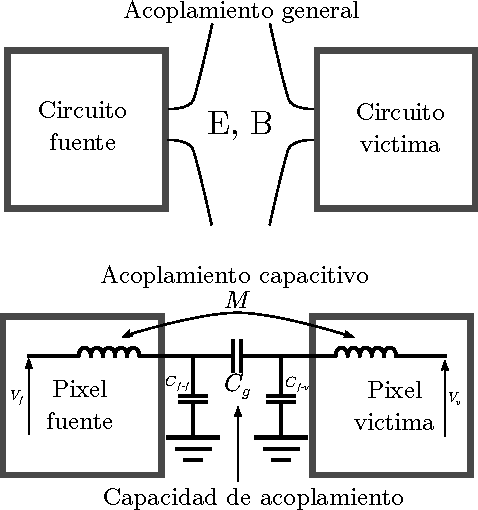
\includegraphics[width=0.4\textwidth]{Modelado/AcoplamientoCapacitivoGeneral.pdf}
	\caption{Modelo de acoplamiento capacitivo entre dos \textit{pixeles}.}
	\label{fig:acoplamiento-capacitivo-modelo}
\end{figure}


En el mismo sentido, debido a que el efecto capacitivo de placas planas paralelas enfrentadas (relacionado a la capacidad de \textit{fringe}) es mucho mayor al de placas planas paralelas coplanares (relacionada a la capacidad entre islas metálicas cercanas), se puede considerar que el acoplamiento es de tipo capacitivo débil \cite{Tesche:EMC} (donde no se considerarán efectos de re-acoplamiento y acoplamiento inverso), lo que permite utilizar un modelo simplificado de acoplamiento, considerando fuentes controladas de corriente, mostrado en la figura \ref{fig:circuito-equivalente-acoplamiento-capacitivo-debil}. Los valores de las fuentes controladas se muestran en la ecuación \ref{eq:expresiones-fuentes-controladas}, aunque en términos prácticos el valor de $M$, la inductancia mutua, se despreciará, por lo que no existirá una fuente controlada de tensión.

\begin{subequations}
	\label{eq:expresiones-fuentes-controladas}
	\begin{align}
		i' = j \omega C_g v_f \\
		v' = j \omega M i_f \approx 0
	\end{align}
\end{subequations}

\begin{figure}[htp]
	\centering
	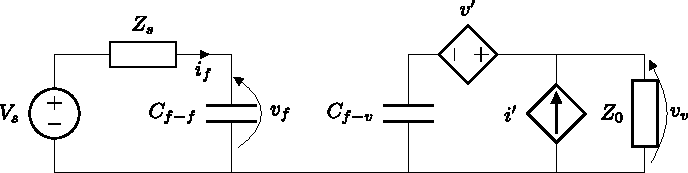
\includegraphics[width=0.8\textwidth]{Modelado/AcoplamientoCapacitivoDebil.pdf}
	\caption{Circuito equivalente del modelo de acoplamiento capacitivo débil, utilizando fuentes de corriente, para una carga de impedancia igual a la impedancia característica de la línea de transmisión conectada.}
	\label{fig:circuito-equivalente-acoplamiento-capacitivo-debil}
\end{figure}

Para adaptar este circuito al modo de funcionamiento de TLM, es posible considerar a la fuente de corriente y el capacitor de \textit{fringe} como un equivalente Norton, y convertirlo en un equivalente Thévenin, de modo que la tensión desarrollada sobre $Z_0$, y por lo tanto, la tensión transmitida al nodo correspondiente al \textit{pixel} víctima, resulte de un divisor resistivo:

\begin{align}
	v_v = v_f \frac{C_g}{j\omega C_{f-v}} \frac{Z_0}{Z_0 + \frac{1}{j\omega C_{f-v}}}
\end{align}

% Podría haber un delay?

La tensión $v_f$ es la que desarrolla el capacitor de \textit{fringe} del \textit{pixel} fuente. Utilizando consideraciones similares, el efecto de este capacitor para el circuito fuente se podría obtener, para el acoplamiento capacitivo, como el paralelo de la capacidad de \textit{fringe} fuente con el circuito que lo conecta al circuito víctima. Sin embargo, dado que, como se dijo antes, la capacidad $C_g$ es mucho menor a las capacidades de \textit{fringe}, $C_{f}$, los efectos del circuito víctima y de la capacidad de acople son despreciables. De esta forma, el valor del coeficiente de reflexión resulta:

\begin{align}
	\rho =  \left| \frac{1/(j\omega C_{f-f}) - Z_0}{1/(j\omega C_{f-f}) + Z_0} \right|
\end{align}

Se debe tener en cuenta que, dado que la señal recorre un camino de $\Delta l / 2$ desde el nodo hasta el capacitor de \textit{fringe}, el cálculo de la tensión reflejada se debe realizar en $n\Delta t/2$. Esto es porque en el tiempo siguiente, exactamente un $\Delta t$ luego de enviada la señal, la tensión reflejada debe impactar en el nodo original, como se esquematizó sobre el \textit{pixel} metálico de la figura \ref{fig:modelo-con-lineas-de-transmision}.

El resultado arrojado por la simulación será un archivo, de formato \textsc{.npy}, que es una matriz tridimensional, que puede ser considerada como un apilamiento, de tamaño igual a la cantidad de tiempos simulados, de matrices bidimensionales con tamaño igual al de la estructura, como se muestra en la figura \ref{fig:EstructuraTiemposMatrizNumpy}. En cada una de estas matrices bidimensionales, cada elemento posee un valor, que no es más que la tensión vista en ese nodo en el tiempo al que la matriz bidimensional corresponde en la estructura tridimensional creada. De ser necesario, se pueden establecer los parámetros de una ventana de Hanning para disminuir el comportamiento espúreo de alta frecuencia debido a la limitación en tiempo de la señal de salida.

\begin{figure}[h]
	\centering
	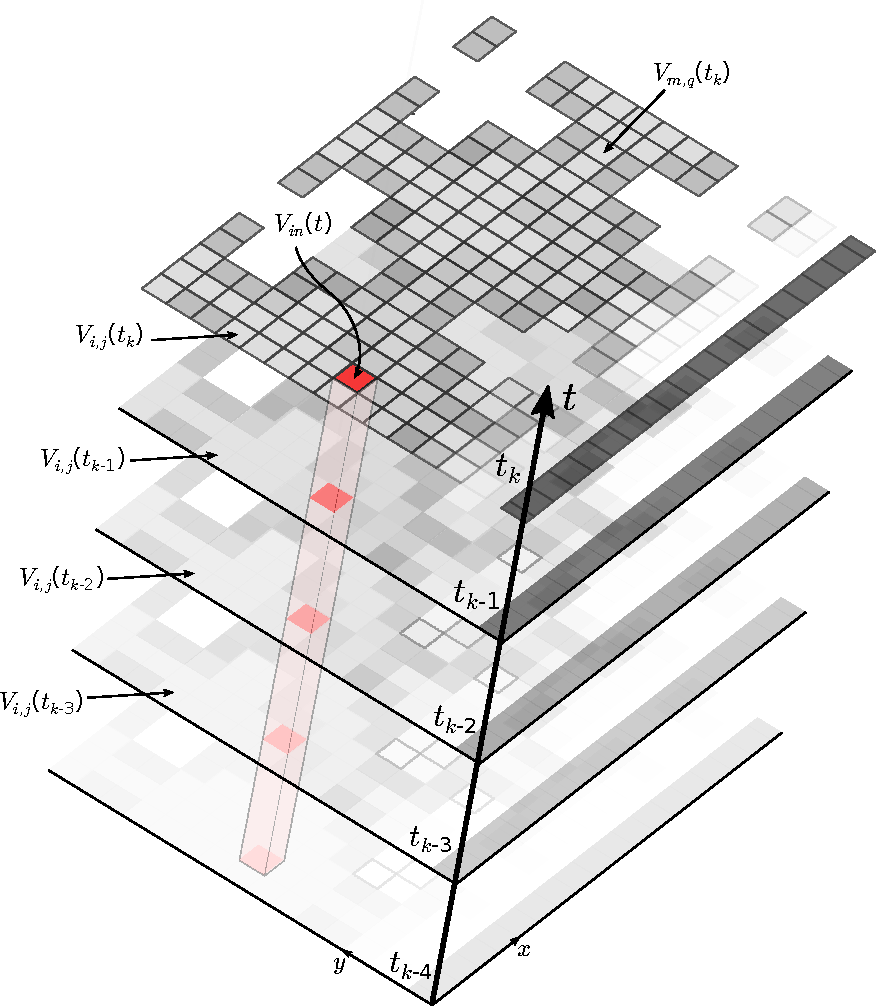
\includegraphics[width=0.9\textwidth]{Modelado/ConceptoMatrizProgresoTiempo.pdf}
	\caption{Estructura de la matriz que se guarda y se lee del disco rígido. La estructura posee todas las tensiones calculadas para cada tiempo y para cada pixel en particular.}
	\label{fig:EstructuraTiemposMatrizNumpy}
\end{figure}

El análisis de la tensión del nodo de salida, teniendo en cuenta la tensión del nodo de entrada aplicada, da lugar a una transferencia de tensión.